\documentclass[a4paper,11pt,fleqn]{article}

\usepackage[french]{babel}
\usepackage[utf8x]{inputenc}
\usepackage{url}
\usepackage[T1]{fontenc}

\usepackage[toc,page]{appendix}

\usepackage{graphicx}


\begin{document}

\title{Master Web Intelligence 2A 2012-2013 \\
Ubiquitous Computing\\ TP Context-Awareness\\}
\author{Christophe Gravier\\
\texttt{christophe.gravier@telecom-st-etienne.fr}\\
\texttt{@chgravier}}

\date{}
\maketitle

\tableofcontents

\newpage

\section*{Préambule}
Ce travail pratique fait suite aux deux séances précédentes. Nous nous plaçons toujours dans le cas d'usage des capteurs de température et de luminosité pour piloter des volets. Vous avez du mettre en \oe{}uvre la partie hardware Arduino (avec X. Serpaggi) et communication (avec J.P. Jamont). Nous allons mettre en place le serveur de contexte, et vous mettrez en \oe{}uvre l'aspect mobilité (avec J. Stan).\\

\fbox{

\parbox{0.9\linewidth}{
Vous devez rendre un compte rendu de TP au format PDF. Ce compte-rendu comportera vos réponses aux questions posées dans ce document, ainsi que les portions de code que vous jugez importante en réponse à ces questions. Ce document sera envoyé à l'adresse : \textbf{wiuclab@gmail.com} avant \textbf{le 31 janvier 2013 23:59}, en indiquant dans le nom de l'archive ainsi que dans le corps du mail les noms et prénoms du binôme. Vous pouvez également adjoindre dans le corps du message, ou envoyer \textit{a posteriori} vos remarques/commentaires et suggestions d'amélioration de ce TP à la même adresse (tout commentaire constructif bienvenu !)
}
}

\section{Description du TP}
Concernant la partie mise en \oe{}uvre pour le "serveur de contexte", il nous faut faire le lien entre les Arduino d'un côté, et les clients Android de l'autre. Les contraintes technologiques sont donc :
\begin{itemize}
 \item côté Arduino : les données sont exposées via un serveur HTTP qu'il faut "moissoner" (les Arduino ne poussent pas l'information, cf. fonctionnement TP Arduino).
 \item côté Android : le client doit être écrit en Java, afin de recevoir les notifications de changement de contexte.
\end{itemize}


\'{E}tant donné que :

\begin{enumerate}
 \item vous n'avez plus un accès aisé aux Arduino
 \item tout le monde n'a pas terminé les TPs précédents (?)
\end{enumerate}

Nous avons le besoin de nous munir d'un simulateur de ces données de contexte (un serveur Web qui simulera celui embarqué dans les Arduinos). Plusieurs logiciels s'offrent à nous (Amigo\footnote{\url{http://www.hitech-projects.com/euprojects/amigo/}}, Siafu\footnote{\url{http://siafusimulator.sourceforge.net/}}, etc.). Le problème de ces logiciels pour notre TP est qu'ils sont complexes et long à prendre en main (nous n'avons que 4h !).\\

Je vous ai donc préparé un serveur en javascript utilisant node.js\footnote{\url{http://nodejs.org/}} et faye\footnote{\url{http://faye.jcoglan.com/node.html}} qui :
	\begin{itemize}
		\item génère toutes les 3 secondes des nouvelles valeurs (aléatoirement) de température et de luminosité
		\item stocke la valeur opened/closed pour les volets dans un fichier
		\item sert au client, en réponse à une requête HTTP GET, les valeurs temperature, luminosité et état des volets en JSON (consultation du contexte)
		\item sert de serveur de publish/subscribe pour des clients compatibles avec le protocole bayeux\footnote{\url{http://svn.cometd.com/trunk/bayeux/bayeux.html}}
		\item fait des publications toutes les 3 secondes du triple (temperature, luminosité, volets) comme les deux premières sont susceptibles d'avoir changées sur un topic dédié.
	\end{itemize}

La première étape sera d'installer mon serveur sur votre machine (c.f. liste des tâches plus loin).

\vspace{1cm}

\textbf{Tout le code et documentation dont vous disposez est accessible sur \url{https://github.com/cgravier/WI-UCLab}.}\\


\section{Compréhension de l'architecture}\label{sec:understand}

Nous allons implémenter l'architecture présentée à la figure~\label{fig:archi}.
La partie entourée correspond à ce qui est traité durant ce TP, avec de part et d'autre ce que vous avez déjà réalisé et ce que vous réaslierez dans le prochain TP.

\begin{figure}
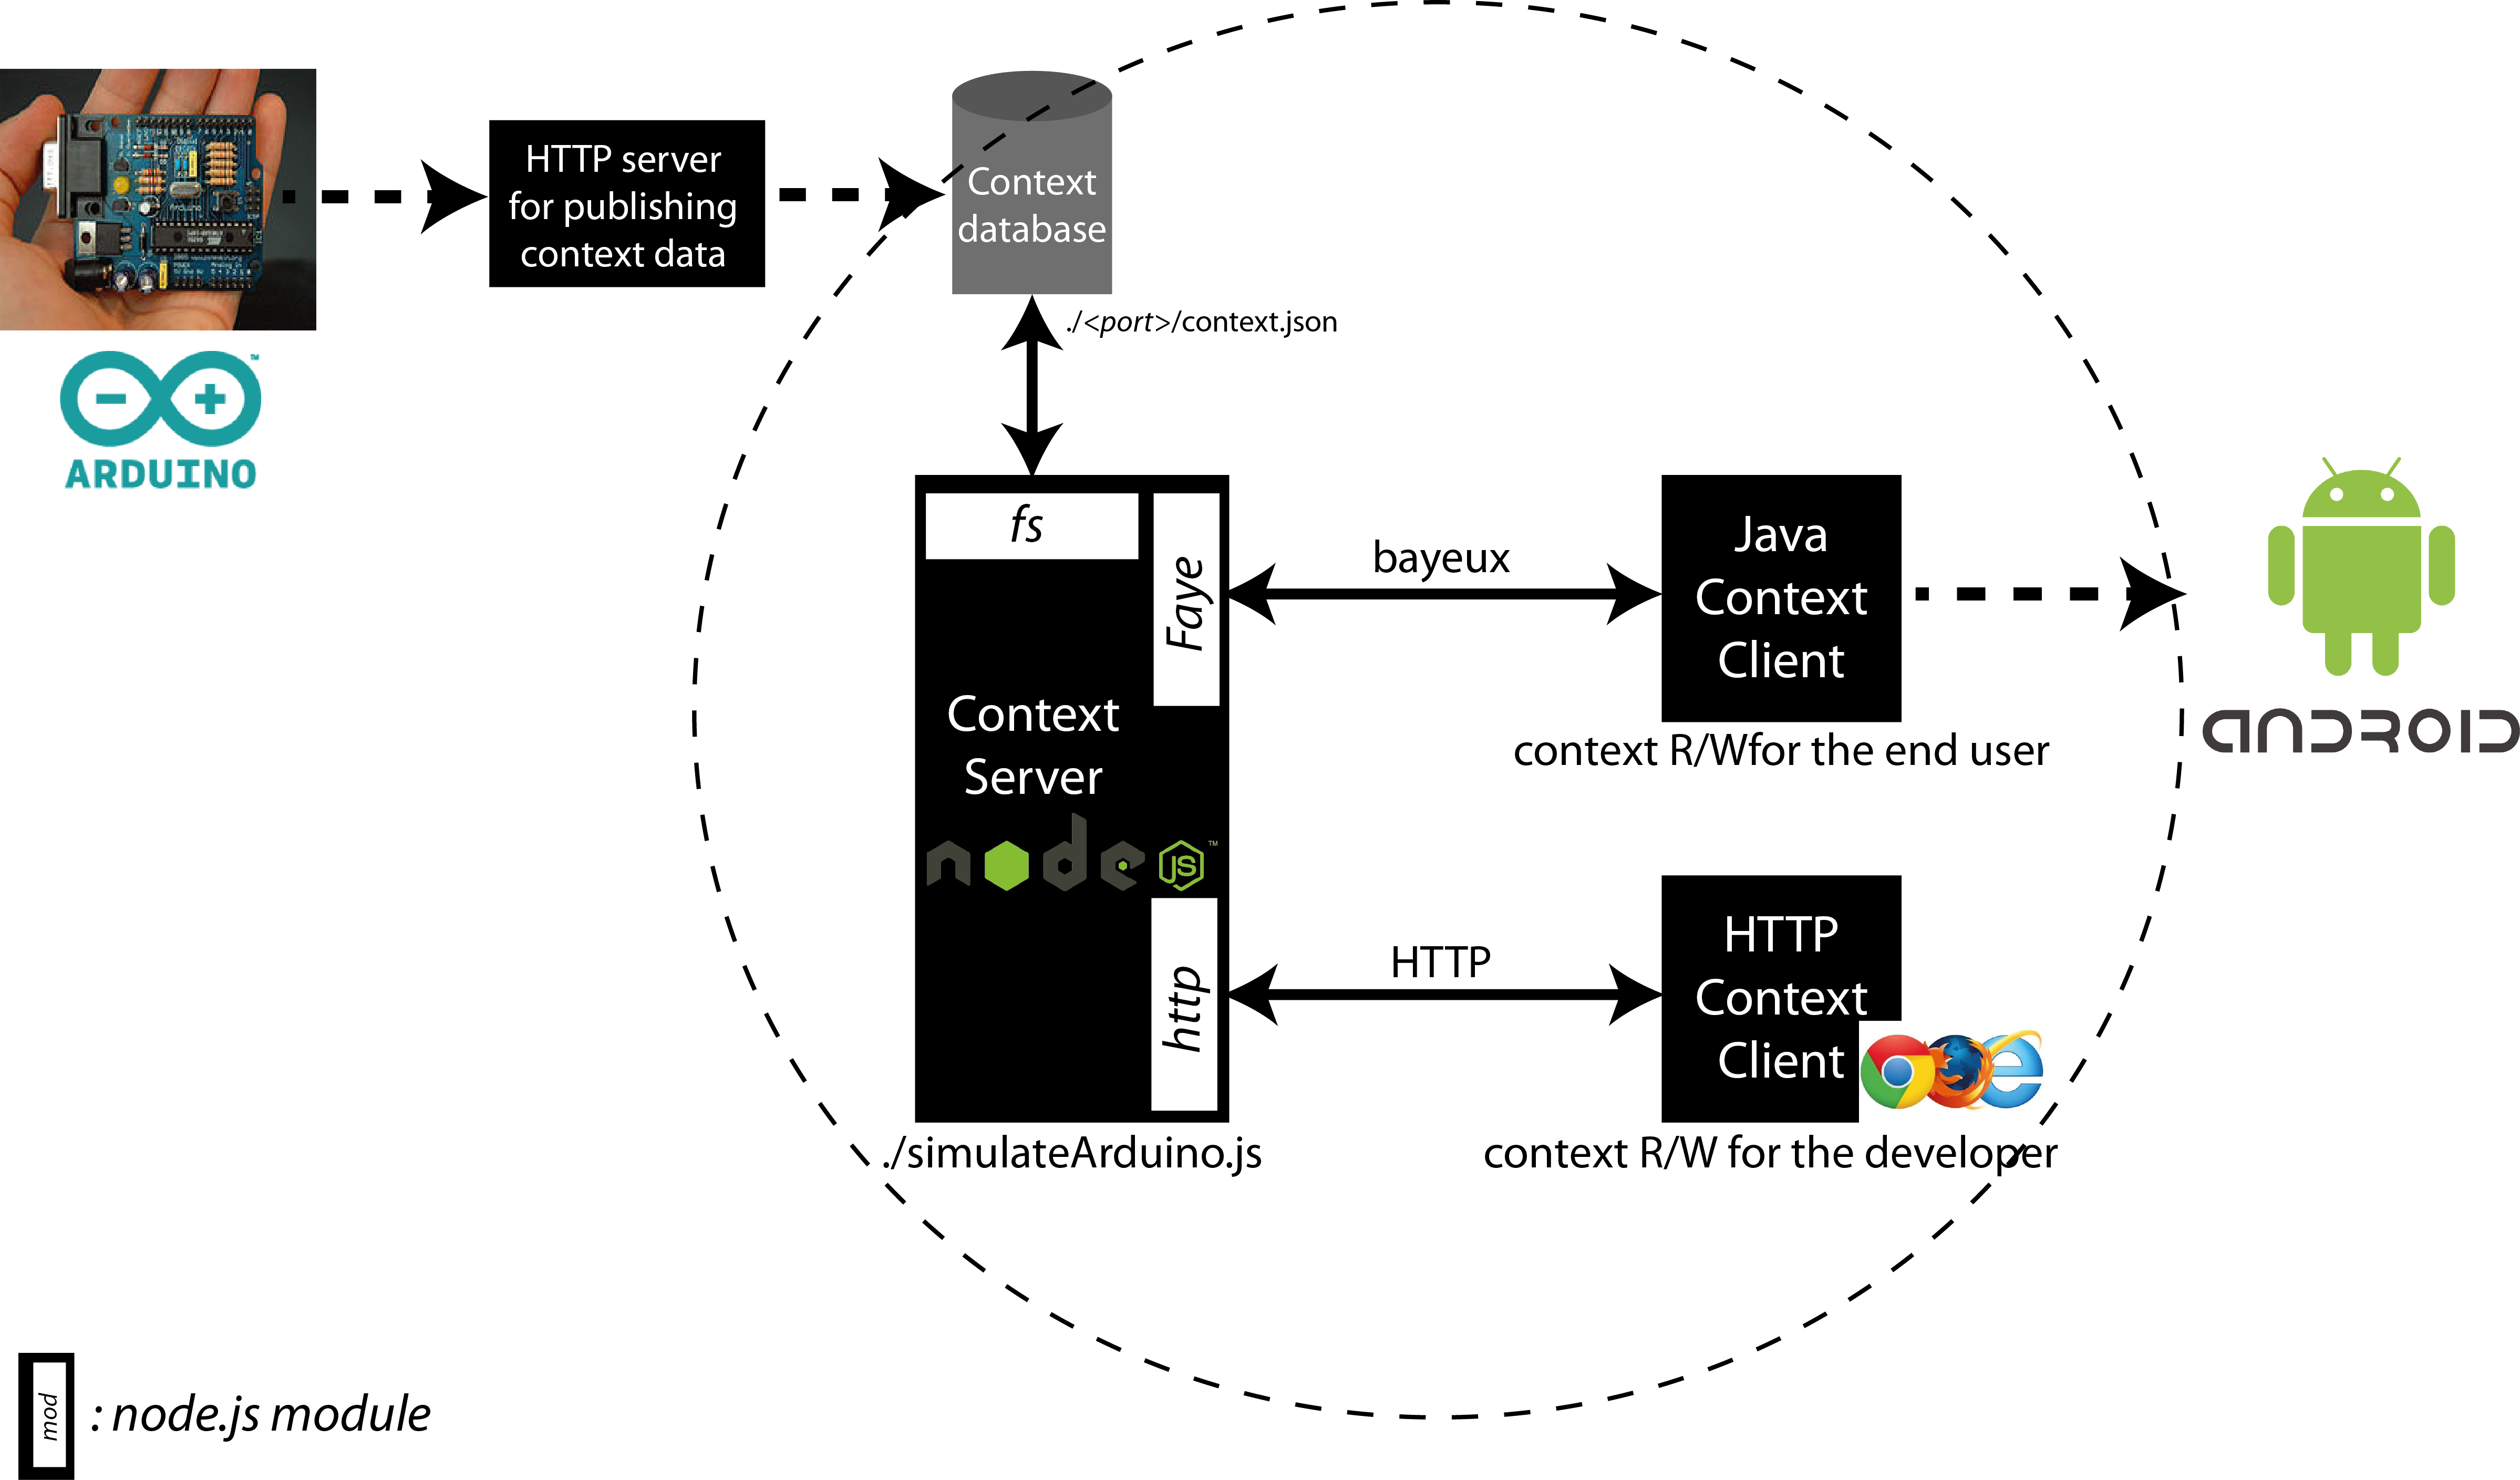
\includegraphics[width=\textwidth]{./img/archi.png}
\caption{Architecture déployée durant ce TP.}
\end{figure}
\vspace{10pt}

\textbf{Traval demandé} : se document sur le Web et répondre aux questions suivantes :
\begin{enumerate}
	\item Qu'est-ce que le protocole Bayeux ?
	\item Qu'est-ce que node.js ?
	\item Qu'est-ce que le module Faye pour node.js ?
\end{enumerate}


\section{Installation et configuration du serveur de contexte}\label{sec:installandrun}

Dans cette partie nous nous intéressons à l'installation et à la configuration du serveur de contexte.\\

\textbf{Traval demandé} : Les étapes du travail à réalier sont les suivantes :
\begin{enumerate}
	\item Installer node.js\footnote{\url{http://nodejs.org/}}.
	\item Télécharger le serveur écrit en javascript\footnote{\url{https://github.com/cgravier/WI-UCLab/blob/master/context-server-nodejs/simulateArduino.js}}. 
	\item Installer les modules nécessaies à node.js pour exécuter le serveur (parcourir les dix premières lignes du code source peut se révêler intelligent).
	\item Décider d'un numéro de port ($>1024$, par exemple 8081) sur lequel votre serveur écoutera.
	\item Dans le répertoire contenant le script du serveur, créer un sous répertoire portant comme nom votre numéro de port
	\item Lancer le serveur (les instructions sont dans le fichier README).
\end{enumerate}

Lorsque votre serveur est en cours d'exécution, il sait sait répondre à deux types de requêtes sur le port choisi :
\begin{itemize}
	\item Requêtes HTTP GET : nous l'utiliserons pour consulter l'état du contexte dans le navigateur Web.
	\item Requêtes conforme au protocole bayeux: note client Java utilisera ce protocole.
\end{itemize}
\vspace{10pt}

Vous pouvez vérifier le bon fonctionnement de votre serveur en accédant dans votre navigateur à l'adresse : \url{http://<votreip>:<votreport>}. Tester l'accès au serveur en HTTP via un navigateur:
	\begin{itemize}
		\item Récupérer les valeurs température, luminosité et état des volets en JSON,
		\item Ouvrir et refermer les volets à l'aide de requêtes HTTP GET.
	\end{itemize}

Les données sont publiées toutes les 3 secondes. Si vous refaite une requête après 3 secondes, vous pourrez constater que le contexte évolue au cours du temps, mais que les volets restent ouverts ou fermés tant que vous n'avez pas agit. Automatiser l'ouverture et la fermeture des volets fait l'objet de la suite de ce travail.


\section{Client réactif aux modifications de contexte en Java}\label{sec:coding}


\subsection{Coder un client standalone Java au serveur}

\textbf{Traval demandé} :
\begin{enumerate}
\item \`{A} l'aide des bibliothèques listées et accessibles sur le compte git mentionné précédemment, écrire un client standalone Java au serveur.
\item La principale bilbiothèque à s'approprier est CometD, une bibliothèque permettant de se connecter en Java (entre autre) à un serveur Bayeux \url{http://cometd.org/}
\item Tester l'accès au serveur via le client Java (confronter que le client Java et votre navigateur récupèrent les mêmes valeurs).
\end{enumerate}
Notez bien que lire les fichiers README est toujours utile.

\subsection{Mise en \oe{}uvre d'un début de context-awareness}

\textbf{Traval demandé} :
\begin{enumerate}
 \item Modifier le client Java pour prendre des décisions et réaliser l'action automatiquement d'ouvrir/fermer les volets suivant certains seuils de sensibliité au contexte:
	\begin{itemize}
		\item fermer les volets si la température descend en dessous de 15 degrés  (il fait trop froid !) ou la luminosité dépasse 1500 lux (trop de lumière !).
		\item ouvrir les volets si la température dépasse 25 degrés (il fait trop chaud !) ou la luminosité descend en dessous de 800 lux (pas assez de lumière!).
	\end{itemize}
Dans le cas où il fait plus de 25 degrés mais avec une luminosité de plus de 1500 lux, ou encore que la température est inférieure à 15 degrés mais avec une luminosité de plus de moins de 800 lux, l'arbitrage est de laisser les volets fermés.
\item Compiler et vérifier que cela fonctionne !
\end{enumerate}

\subsection{Impliquer l'utilisateur}
Dans les systèmes sensibles au contexte, il est quelques fois difficile de prendre des décisions à la place de l'utilisateur. Dans le cas des volets, bien que la température ou la luminosité franchissent certains seuils, il est possible que l'utilisateur souhaite conserver l'état ouvert ou fermé de ses volets.\\

\begin{itemize}
 \item Modifier le client standalone Java en ajoutant une fenêtre modale pour permettre de confirmer ou d'infirmer le fait d'ouvrir ou fermer les volets (en cas de changement d'état).
 \item Il est difficile de demander à l'utilisateur systématiquement son avis (notamment lorsque les valeurs oscillent autour des seuils de manière permanente). Ainsi, lorsque le système aura sollicité l'utilisateur et quelque soit sa réponse, le système ne changera plus l'état des volets et ne sollicitera plus l'utilisateur pour la prochaine heure\footnote{Pour les besoins du tests, fixer ce temps d'attente à 30 secondes}.
\end{itemize}


\section{Client proactif aux modifications de contexte en Java}\label{sec:thinkharder}
Jusqu'à maintenant, nous nous sommes bornés à réagir à des changements de contexte. De tels systèmes vont quelques fois jusqu'à anticiper le changement. C'est ce que nous allons étudier dans cette dernière partie du TP.\\
Nous nous plaçons dans la configuration où un utilisateur ouvre et ferme manuellement ses volets. Nous nous contentons de consigner toutes les deux heures : la valeur de la température, la valeur de la lumisoité,  l'état des volets, et l'heure de la journée. Nous procédons à ces observations pendant 3 mois. Nous disposons donc de 1080 observations. Nous souhaitons maintenant mettre en oevure une approche qui permettra de déployer un système dédié à notre utilisateur pour anticiper l'ouverture et la fermeture de ses volets, suivant son habitude.\\

\textbf{Traval demandé} :
\begin{enumerate}
	\item Proposer une approche qui permettrait d'adresser ce problème (1 page).
\end{enumerate}

\section{Optionnel : proposer une modification du serveur de simulation de données de contexte}
Le serveur génère des données fictives, pris de manière aléatoire entre 0 et 40 degrés pour la température et 0 et 2000 lux pour la luminosité. Rien n'empêche le simulateur de donner une température de 3 degrés, suivi 3 secondes plus tard d'une température de 37 degrés !
\begin{itemize}
 \item Modifier le serveur pour générer des valeurs plus plausibles. Idéalement votre proposition est paramétrable (i.e. ne pas coder avec les pieds !).
\end{itemize}


%Pour être plus utile pour le TP android :
%\subsection{Expliquer les décisions à l'utilisateur}
%On se replace ici dans le cs d'un scénario sans interaction utilisateur.
%
%\begin{itemize}
% \item \`{A} l'aide de Google C2DM (Android Cloud to Device Messaging Framework) \url{http://code.google.com/intl/fr-FR/android/c2dm/}, mettre en place des notifications utilisateur pour lui dire que ses volets ont été ouverts/fermés automatiquement et pourquoi (température et/ou luminosité trop haute).
%\end{itemize}


\section{Wrap-up}

Dans ce TP nous avons essayé de détourer la notion de contexte. Nous avons vu que le contexte était :
\begin{itemize}
	\item évolutif dans le temps,
	\item issu de données hétérogènes,
	\item quelque fois subit (température ou luminosité ici) ou piloté (volets ouverts/fermés).
\end{itemize}

Vous vous êtes heurtés à des difficultés de différents ordres pour mené à bien la gestion du contexte dans l'applicaiton qui nous intéresse ici. Une première partie de ces difficultés est en fait d'ordre scientifique pour les chercheurs dans ce domaine, à savoir :
\begin{itemize}
	\item comment modéliser le contexte ?
	\item comment réagir à des changements de la manière la plus pertinente et transparente pour l'utilisateur ?
	\item comment gérer de manière individuelle le contexte ?
	\item comment prédire des changements de contexte significatifs pour que le système devienne ubiquitaire ?
	\item comment justifier les actions du système auprès de l'utilisateur ? (facile en cas de règle métier, quid lorsque l'on apprend un modèle ?)
	\item comment conduire des inférences sur les données de contexte ?
\end{itemize}

Bien entendu ces problèmes sont intimement connecté avec les considérations technologiques associées à la gestion de contexte, puisque le contexte est :
\begin{itemize}
	\item centré sur le Web.
	\item dépendant du middleware sous-jacent.
\end{itemize}


\end{document}